%%%% Modèle proposé par kira.ribeiro@universite-paris-saclay.fr  %%%%
%%%% màj : 27/01/2023 %%%%

\documentclass[french,12pt,a4paper]{book}
\usepackage[utf8]{inputenc}
\usepackage[T1]{fontenc}
\usepackage[french]{babel}
\usepackage[default,oldstyle, scale=.95]{opensans} % police Open Sans
\usepackage{amsmath}
\usepackage{stmaryrd}
\usepackage{amsfonts}
\usepackage{amssymb}
\usepackage{booktabs}
\usepackage{algorithm2e}
\SetKwInOut{KwAttr}{Attribute}
\usepackage{caption}
\captionsetup[figure]{font=small,labelfont=small}
\usepackage{xcolor} % où color selon l'installation
\definecolor{Prune}{RGB}{99,0,60} % l14-33 : couleurs de la charte graphique upsaclay
\definecolor{B1}{RGB}{49,62,72} 
\definecolor{C1}{RGB}{124,135,143}
\definecolor{D1}{RGB}{213,218,223}
\definecolor{A2}{RGB}{198,11,70}
\definecolor{B2}{RGB}{237,20,91}
\definecolor{C2}{RGB}{238,52,35}
\definecolor{D2}{RGB}{243,115,32}
\definecolor{A3}{RGB}{124,42,144}
\definecolor{B3}{RGB}{125,106,175}
\definecolor{C3}{RGB}{198,103,29}
\definecolor{D3}{RGB}{254,188,24}
\definecolor{A4}{RGB}{0,78,125}
\definecolor{B4}{RGB}{14,135,201}
\definecolor{C4}{RGB}{0,148,181}
\definecolor{D4}{RGB}{70,195,210}
\definecolor{A5}{RGB}{0,128,122}
\definecolor{B5}{RGB}{64,183,105}
\definecolor{C5}{RGB}{140,198,62}
\definecolor{D5}{RGB}{213,223,61}
\usepackage{mdframed}
\usepackage{multirow} %% Pour mettre un texte sur plusieurs rangées
\usepackage{multicol} %% Pour mettre un texte sur plusieurs colonnes
\usepackage{tikz}
\usepackage{graphicx}
\usepackage[absolute]{textpos} 
\usepackage{colortbl}
\usepackage{array}
\usepackage{geometry}
\usepackage{titlesec}
\usepackage{dsfont}
\setcounter{secnumdepth}{3}
\usepackage{hyperref}
\hypersetup{ % paramétrage couleur des liens hypertextes, toujours garder colorlinks=true
    colorlinks=true,
    linkcolor=black,
    urlcolor=A5}

\usepackage[
    backend=biber,
    style=numeric,
    natbib=true,
    sorting=none
]{biblatex}

\addbibresource{Biblio.bib}

\renewcommand{\FrenchLabelItem}{\textbullet}
\renewcommand{\topfraction}{0.85}     % Autorise les images à occuper 85% du haut de page
\renewcommand{\bottomfraction}{0.9}   % Autorise les images à occuper 70% du bas de page
\renewcommand{\textfraction}{0.10}    % Demande seulement 15% de texte minimum par page
\renewcommand{\floatpagefraction}{0.80}% Une page isolée n'est créée que si l'image occupe au moins 60% de l'espace

\DeclareMathOperator*{\argmax}{arg\,max}
\DeclareMathOperator*{\argmin}{arg\,min}

\pagestyle{plain} % pour ne garder que les n°de page en milieu-bas et supprimer les indications de chapitre en marge haute

\begin{document}

\begin{titlepage}

%\thispagestyle{empty}

\newgeometry{left=6cm,bottom=2cm, top=1cm, right=1cm}

\tikz[remember picture,overlay] \node[opacity=1,inner sep=0pt] at (-13mm,-135mm){
\includegraphics{Frame-ups.pdf}};

%*****************************************************
%******** NUMÉRO D'ORDRE DE LA THÈSE À COMPLÉTER *****
%******** POUR LE SECOND DÉPOT                   *****
%*****************************************************

\color{white}

\begin{picture}(0,0)
\put(-152,-743){\rotatebox{90}{\Large \textsc{THESE DE DOCTORAT}}} \\
\put(-120,-743){\rotatebox{90}{NNT : 2020UPASA001}}
\end{picture}
 
%*****************************************************
%******************** TITRE **************************
%*****************************************************

\flushright
\vspace{10mm} % à régler éventuellement
\color{Prune}

\fontsize{22}{26}\selectfont
  \Huge Accélération d'un environnement de simulation de mesures de soutien électronique par l'intelligence artificielle \\

\normalsize
\color{black}
\Large{\textit{Accelerating an electronic support measures simulation environment using artificial intelligence}} \\
%*****************************************************


\fontsize{8}{12}\selectfont

\vspace{1.5cm}

\normalsize
\textbf{Thèse de doctorat de l'université Paris-Saclay} \\

\vspace{6mm}

\small École doctorale n° 580, Sciences et technologies de l'information et de la communication (STIC)\\
\small Spécialité : Sciences du traitement du signal et des images\\
\small Graduate School : Ecole Graduée Informatique et Sciences du Numérique. Référent : ENS Paris-Saclay \\
\vspace{6mm}

\footnotesize Thèse préparée dans l'unité de recherche Laboratoire SATIE (UMR 8029), sous la direction de Thomas RODET, Professeur des universités, et la co-supervision de Cyrille ENDERLI, Ingénieur de recherche (Thales DMS), tuteur en entreprise. \\
\vspace{15mm}

\textbf{Thèse soutenue à Paris-Saclay, le 25 octobre 2026, par Matthieu CORNU}\\
\bigskip
\Large {\color{Prune} \textbf{Matthieu CORNU}}

%************************************
\vspace{\fill} % ALIGNER LE TABLEAU EN BAS DE PAGE
%************************************

\bigskip

\flushleft
\small {\color{Prune} \textbf{Composition du jury}}\\
{\color{Prune} \scriptsize {Membres du jury avec voix délibérative}} \\
\vspace{2mm}
\scriptsize
\begin{tabular}{|p{7cm}l}
\arrayrulecolor{Prune}
\textbf{Michèle GOUIFFES} &   Présidente\\ 
Professeure des universités, Université Paris-Saclay, IUT ORSAY & \\
\textbf{Jean Marc LE CAILLEC} &  Rapporteur \\ 
Professeur des universités, IMT Atlantique Brest   &   \\ 
\textbf{Bruno SIXOU} &  Rapporteur \\ 
Maître de conférences, Insa Lyon  &   \\ 
\textbf{Michèle GOUIFFES} &  Examinatrice \\ 
Professeure des universités, Université Paris-Saclay, IUT ORSAY &   \\ 
\textbf{Thomas HOURET} &  Examinateur \\ 
Ingénieur de recherche, ONERA   &   \\ 
 

\end{tabular} 

\end{titlepage}


% page des résumés à garder en 2ème page. Si les résumés sont trop longs pour tenir sur une seule et même page, on peut mettre un résumé par page
\thispagestyle{empty}
\newgeometry{top=1.5cm, bottom=1.25cm, left=2cm, right=2cm}


\noindent 
%*****************************************************
%***** LOGO DE L'ED À CHANGER IMPÉRATIVEMENT *********
%*****************************************************

\includegraphics[height=2.45cm]{logo_usp_STIC.png}
\vspace{1cm}
%*****************************************************

\small

\begin{mdframed}[linecolor=Prune,linewidth=1]

\textbf{Titre:} Accélération d'un environnement de simulation de mesures de soutien électronique par l'intelligence artificielle

\noindent \textbf{Mots clés:} Guerre électronique, ESM, Simulation, Intelligence Artificielle, Transformer, Traitement de séquences

\vspace{-.5cm}
\begin{multicols}{2}
\noindent \textbf{Résumé:} L'histoire de la guerre moderne est indissociable de la maîtrise du spectre électromagnétique. Dans la guerre électronique aéroportée, le capteur de Mesures de Soutien Électronique (ESM) opère pour intercepter les émissions radar. La validation des algorithmes de post-traitement exploitant ces interceptions s'appuie sur la simulation numérique. Cependant, les environnements virtuels de référence sont limités par la lenteur de leurs modules de Détection et Caractérisation des Impulsions (DCI).

L'objectif de cette thèse est d'accélérer un environnement virtuel de référence en substituant le module DCI par un modèle d'intelligence artificielle. La problématique s'apparente à un défi de modélisation d'un algorithme de traitement de séquences. Pour pallier la complexité du système réel, un environnement d'étude contrôlé (DCIS) est d'abord élaboré. La viabilité de l'approche est évaluée sur un problème d'ordonnancement supervisé, établissant la supériorité de l'architecture Transformer.  

L'approche principale consiste ensuite en une transduction Séquence-vers-Séquence. Bien que l'approche soit validée sur des séquences courtes, le passage à l'échelle via un fenêtrage dynamique révèle des failles. Pour y remédier, une reformulation causale du problème est appliquée par sérialisation événementielle des données. 
\end{multicols}

\end{mdframed}

\begin{mdframed}[linecolor=Prune,linewidth=1]

\textbf{Title:} Accelerating an electronic support measures simulation environment using artificial intelligence

\noindent \textbf{Keywords:} Electronic Warfare, ESM, Simulation, Artificial Intelligence, Transformer, Sequence Processing

\begin{multicols}{2}
\noindent \textbf{Abstract:} The history of modern warfare is inseparable from the mastery of the electromagnetic spectrum. In airborne electronic warfare, the Electronic Support Measures (ESM) sensor operates to intercept radar emissions. The validation of the post-processing algorithms using thoses datas relies on numerical simulation. However, standard virtual environments are limited by the slowness of their Pulse Detection and Characterization (DCI) modules.

The objective of this thesis is to accelerate a standard virtual environment by replacing the DCI module with an artificial intelligence model. The problem is formalized as a challenge of modeling a sequence processing algorithm. To overcome the complexity of the real system, a controlled study environment (DCIS) is first developed. The viability of the approach is evaluated on a supervised sorting problem, establishing the superiority of the Transformer architectur.  

The main approach then consists of a Sequence-to-Sequence transduction. While the approch is validated on short sequences, scaling up via dynamic windowing revealsn some weaknesses. To address this, a causal reformulation of the problem is applied through the event-based serialization of the data. 
\end{multicols}
\end{mdframed}

% --- Chapitre : Dominant et coloré ---
\titleformat{\chapter}[hang]{\bfseries\huge\color{Prune}}{\thechapter\ -}{1ex}{}
\titlespacing{\chapter}{0pc}{0ex}{2pc}

% --- Section : Grand et Gras ---
\titleformat{\section}[hang]{\bfseries\Large}{\thesection\ .}{0.5em}{}
\titlespacing{\section}{0pc}{3.5ex plus 1ex minus .2ex}{2.3ex plus .2ex}

% --- Subsection : Taille Normale et Gras ---
\titleformat{\subsection}[hang]{\bfseries\normalsize}{\thesubsection\ .}{0.5em}{}
\titlespacing{\subsection}{1.5pc}{2.5ex plus 1ex minus .2ex}{1.5ex plus .2ex}

% --- Subsubsection : Taille Normale, Italique (ou Small Caps) avec plus de retrait ---
\titleformat{\subsubsection}[hang]{\itshape\normalsize}{\thesubsubsection\ .}{0.5em}{}
\titlespacing{\subsubsection}{3pc}{1.5ex plus .5ex minus .2ex}{1em}

%\titleformat{\chapter}[hang]{\bfseries\Large\color{Prune}}{\thechapter\ -}{.1ex}
%{\vspace{0.1ex}
%}
%[\vspace{1ex}]
%\titlespacing{\chapter}{0pc}{0ex}{0.5pc}
%
%\titleformat{\section}[hang]{\bfseries\normalsize}{\thesection\ .}{0.5pt}
%{\vspace{0.1ex}
%}
%[\vspace{0.1ex}]
%%\titlespacing{\section}{1.5pc}{4ex plus .1ex minus .2ex}{.8pc}
%
%\titleformat{\subsection}[hang]{\bfseries\small}{\thesubsection\ .}{1pt}
%{\vspace{0.1ex}
%}
%[\vspace{0.1ex}]
%%\titlespacing{\subsection}{3pc}{2ex plus .1ex minus .2ex}{.1pc}
%
%\titleformat{\subsubsection}[hang]{\bfseries\small}{\thesubsubsection\ .}{1pt}
%{\vspace{0.1ex}
%}
%[\vspace{0.1ex}]
%%\titlespacing{\subsection}{3pc}{2ex plus .1ex minus .2ex}{.1pc}

\newgeometry{top=4cm, bottom=4cm, left=2cm, right=2cm}

\tableofcontents

\newgeometry{top=4cm, bottom=4cm, left=2.5cm, right=2.5cm}

\include{Introduction}

\include{Problematique}

\include{Etat de l art}

\chapter{Un sujet d'étude pertinent : Module de Détection et Caractérisation des Impulsions Simplifié (DCIS)}
\label{chap:newfocus}
\section{Contexte et motivations}
Lors de nos travaux sur l'évaluation de l'approche sequence-to-sequence (Seq2Seq) pour reproduire les données du DCI, constituant la problématique initiale de ces travaux (Chapitre \ref{chap:prob}), nous nous sommes heurtés à deux obstacles structurels.\\

Le premier réside dans la complexité du traitement opéré par le DCI. Les phénomènes de masquage fréquentiel par repliement de spectre, de saturation des voies d'acquisition, d'intermodulation ou encore la présence d'harmoniques induisent une multitude de facteurs dans la création des artéfacts (illustrés figure \ref{fig:IOex}). Du point de vue de l'apprentissage automatique, cette intrication rend opaque l'identification des causes d'erreur du modèle. Or, la capacité d'isoler la source d'une difficulté, comme diagnostiquer l'incapacité d'une architecture neuronale à modéliser une intermodulation spécifique, est une véritable nécessité méthodologique.\\

Le second obstacle est inhérent à l'exigence de reproductibilité de la recherche scientifique. L'utilisation d'un simulateur industriel impose des contraintes de confidentialité, limitant la diffusion des jeux de données et empêchant la validation indépendante des résultats.  \\

Pour pallier ces limitations, nous proposons un environnement de simulation simplifié, désigné par le terme DCIS (Module de Détection et de Caractérisation des Impulsions Simplifié). Cet outil offre des leviers de contrôle sur les mécanismes générateurs d'artéfacts, facilitant la conception des réseaux de neurones, tout en s'affranchissant des restrictions de diffusion de données industrielles. 


\section{Modélisation systémique du DCIS}
L'architecture du DCIS repose sur deux modules séquentiels aux rôles complémentaires :
\begin{itemize}
\item \textbf{Le générateur stochastique d'environnement :} Ce module régit la succession et la densité des impulsions physiques dans \textbf{le scénario} au fil du temps.
\item \textbf{Le modèle de réception et de suivi:} Ce module simule la dynamique d'acquisition \textbf{du capteur}. Il maintient un état interne (la mémoire de suivi temporel), évalue les détections non-ambiguës (DNA) à chaque instant, et associe ces détections à des pistes.
\end{itemize}  
\; \\

Le cœur de cette modélisation réside dans l'approximation des règles d'extraction des DNA, qui régit l'apparition des artéfacts de masquage. Nous formalisons cette étape avant de détailler la génération de l'environnement et le processus de suivi.  


\subsection{Filtre de Détection Non-Ambiguë (DNA)}
\label{seq:DNA_DCIS}
Dans le système réel, une DNA résulte d'un processus complexe de corrélation de pics d'énergie repliés spectralement sur plusieurs voies. Le DCIS s'abstrait de la notion de repliement matériel pour se concentrer sur un phénomène de masquage par proximité fréquentielle pure. En ajoutant la représentation des contraintes matérielles dans le traitement algorithmique, le DCIS suffit à engendrer des dynamiques d'artéfacts complexes. \\

Considérons un palier temporel contenant $n$ impulsions incidentes $I_1, \dots, I_n$, caractérisées par leurs fréquences $F_1, \dots, F_n$ et leurs niveaux d'énergie $N_1, \dots, N_n$. Nous définissons la matrice de proximité fréquentielle $\mathbf{F} \in \mathbb{R}^{n \times n}$ modélisant la résolution de l'analyse spectrale par un seuil $\delta F$ :
\begin{equation}
\mathbf{F}_{i,j} = \begin{cases}
1 & \text{si } |F_i - F_j| \le \delta F \\
0 & \text{sinon}
\end{cases}
\end{equation} 

Parallèlement, nous établissons la matrice de domination énergétique $\mathbf{L} \in \mathbb{R}^{n \times n}$ :
\begin{equation}
\mathbf{L}_{i,j} = \begin{cases}
1 & \text{si } N_i < N_j \\
0 & \text{sinon}
\end{cases}
\end{equation}

Notre modèle postule qu'une impulsion subit un masquage matériel si une seconde impulsion, à la fois proche en fréquence et de niveau supérieur, est présente simultanément. Puisque $\mathbf{F}$ et $\mathbf{L}$ sont des matrices booléennes, nous calculons la matrice de masquage globale $\mathbf{M}$ via le produit de Hadamard : $\mathbf{M} = \mathbf{F} \odot \mathbf{L}$. Cette opération agit comme un opérateur logique \textbf{ET} : le terme $\mathbf{M}_{i,j}$ vaut $1$ si et seulement si l'impulsion $I_j$ masque l'impulsion $I_i$.  \\

Finalement, une impulsion est promue au statut de DNA si elle n'est masquée par aucune autre, ce qui se traduit par la nullité de la somme sur sa ligne :
\begin{equation}
\text{Sélection}_i= \begin{cases}
\text{Vrai} & \text{si } \sum_{j=1}^{n} \mathbf{M}_{i,j} = 0 \\
\text{Faux} & \text{sinon}
\end{cases}
\end{equation}
Nous noterons cette fonction de filtrage $\mathcal{F}_{\text{DNA}}(\cdot)$ dans la suite de l'étude.

\subsection{Génération de l'environnement : la séquence d'impulsions incidentes}
La première étape de la simulation consiste à synthétiser l'environnement électromagnétique du scénario, c'est-à-dire l'ordre d'arrivée et les caractéristiques des impulsions émises. L'algorithme maintient une densité d'impulsions, définie par le nombre d'impulsions par palier, constante au cours du scénario. Le choix de suppression d'une impulsion du palier actif est aléatoire, régi par une loi de probabilité favorisant la disparition des signaux les plus anciens. Ce processus, détaillé dans l'Algorithme \ref{algo:generation_sequence_scenario}, génère la séquence ordonnée des impulsions émises du scénario, qui sera fournie au deuxième module : la simulation de l'acquisition et du suivi temporel du capteur.  

\begin{algorithm}[htbp]
\DontPrintSemicolon
\SetAlgoLined
\KwIn{Nombre total d'événements $N$, Densité par palier $n$}
\KwOut{Séquence chronologique des paliers $\mathcal{V}_{tot}$, Liste des impulsions incidentes $\mathcal{L}$}
\textbf{Initialisation :} $\mathcal{L} \leftarrow [\,]$, Palier courant $\mathcal{V} \leftarrow [\,]$, Âges $\mathcal{A} \leftarrow [\,]$, $T \leftarrow 0$\;
\vspace{2mm}\tcp*[l]{Générateur stochastique de l'environnement}
\While{$T < N$}{
Générer une nouvelle impulsion $v_{new}$\;
Ajouter $v_{new}$ à la fin de $\mathcal{L}$ et $\mathcal{V}$ \; 
Ajouter l'âge $0$ à la fin $\mathcal{A}$\;
}
\If{$T > n$}{
Soit $m$ la taille de $\mathcal{V}$\;
Sélectionner un indice $k \in [1, m]$ avec probabilité $P(k) = \frac{\mathcal{A}_k + 1}{\sum_{i=1}^{m} \mathcal{A}_i + m}$\;
Extraire $v_k$ de $\mathcal{V}$ et $\mathcal{A}_k$ de $\mathcal{A}$\;
Mettre à jour $v_k$ dans $\mathcal{L}$ avec son âge de clôture $(\mathcal{A}_k + 1)$
}
$T \leftarrow T + 1$\;
Incrémenter tous les éléments de $\mathcal{A}$ de 1\;
\Return $\mathcal{L}$

\caption{Génération stochastique de la séquence d'impulsions incidentes}
\label{algo:generation_sequence_scenario}
\end{algorithm}


\subsection{Simulation de l'acquisition et du suivi temporel}
La seconde étape modélise la dynamique d'acquisition du capteur. Ce module prend désormais en entrée unique la liste globale des impulsions physiques $\mathcal{L}$ générée en amont par l'environnement. Pour traiter ce flux de manière causale et pas-à-pas, le capteur reconstruit dynamiquement le palier actif $\mathcal{V_L}^{(t)}$ à chaque instant de son horloge interne $t$. \\

Une impulsion $v \in \mathcal{L}$ est considérée comme présente sur le palier à l'instant $t$ si sa date d'arrivée ($TOA_v$) est inférieure ou égale à $t$, et que sa date de fin (définie par $TOA_v + LI_v$, où $LI_v$ désigne sa durée) est strictement supérieure à $t$. Ainsi, mathématiquement, l'opération $\mathcal{F}_{\mathcal{V}}$ consistant à construire l'ensemble des impulsions composant le palier courant est définie selon le critère de sélection suivant :
\begin{equation}
\mathcal{F}_{\mathcal{V}}(\mathcal{L}, t) = \mathcal{V_L}^{(t)} = \{ v \in \mathcal{L} \mid TOA_v \le t \text{ et } TOA_v + LI_v > t \}
\end{equation}

Une fois ce palier reconstruit localement, la fonction de filtrage $\mathcal{F}_{\mathrm{DNA}}$ en extrait les détections non-ambiguës. Celles-ci sont ensuite confrontées à la mémoire interne du système (les "pistes"). Ces mémoires sont régulièrement vidées de leurs informations , lesquelles composeront les PDW interceptés par le capteur.\\

Ce processus global intègre les contraintes matérielles du capteur, tel que le nombre de pistes simultanées maximal $N_{max}$,le seuil d'association aux pistes $\delta f$, ou encore de temps de maintien d'une mémoire après sa dernière mise-à-jour $T_{maintien}$, et il est formalisé par l'Algorithme \ref{algo:capteur_process}. 

\begin{algorithm}[httb]
\DontPrintSemicolon
\SetAlgoLined
\KwIn{Séquence d'impulsions incidentes $\mathcal{L}$, Seuil d'association $\delta f$, Maintien $T_{maintien}$}
\KwOut{Séquence des PDW interceptés $\mathcal{R}$}
\textbf{Initialisation :} Temps $t \leftarrow 0$, Pistes actives $\mathcal{P} \leftarrow \emptyset$, Dates de mise à jour $\mathcal{T} \leftarrow \emptyset$, $\mathcal{R} \leftarrow [\,]$\;
\vspace{2mm}\tcp*[l]{Traitement du flux événementiel par le capteur}
\For{$t \leftarrow 1$ \KwTo $T_{\mathrm{max}}$}{
Extraire les DNA : $\mathcal{D} \leftarrow \mathcal{F}_{\text{DNA}}(\mathcal{F}_{\mathcal{V}}(\mathcal{L}, t))$ (Triée par énergie décroissante)\;
\tcp*[l]{1. Association des DNA aux pistes ou création}
\ForEach{impulsion $\mathcal{I} \in \mathcal{D}$ dans l'ordre}{
Chercher la piste active $p \in \mathcal{P}$ vérifiant $\|F_\mathcal{I} - F_{p}\| \le \delta f$ avec la plus haute énergie\;
\eIf{Une piste $p$ valide est trouvée}{
Associer $\mathcal{I}$ à $p$ (mise à jour)\;
Mettre à jour l'âge de suivi associé $t_p \leftarrow t$\;
}{
\If{$|\mathcal{P}| < N_{max}$}{
Créer une nouvelle piste $p_{new}$ à partir de $\mathcal{I}$\;
Ajouter $p_{new}$ à $\mathcal{P}$ et la date $t$ à $\mathcal{T}$\;
}
}
}
\vspace{1mm}
\tcp*[l]{2. Purge de la mémoire et publication}
\ForEach{piste $p \in \mathcal{P}$ par ordre d'énergie décroissant}{
\If{$t - t_p \ge T_{maintien}$}{
Construire le PDW intercepté final à partir de $p$ et $t_p$\;
Ajouter le PDW à la fin de $\mathcal{R}$\;
Retirer $p$ de $\mathcal{P}$ et $t_p$ de $\mathcal{T}$\;
}
}
}
\Return $\mathcal{R}$
\caption{Algorithme d'acquisition, de suivi et de publication des PDW}
\label{algo:capteur_process}
\end{algorithm}

\section{Pertinence de la simulation simplifiée}
Le développement de cet environnement contrôlé répond aux exigences de notre étude (Section \ref{seq:FormaPb}). Bien que structurellement simplifiée, cette modélisation n'entrave pas l'étude des capacités d'apprentissage des réseaux de neurones. La dynamique de transformation opérée par le DCIS reste fondamentalement homologue à celle du capteur réel.\\

Comme l'illustre la Figure \ref{fig:IOsimple}, la projection des séquences incidentes et interceptées met en évidence l'émergence d'artéfacts canoniques (fusions de signaux, disparitions, scissions artificielles, troncatures), identiques à ceux observés sur le DCI (Figure \ref{fig:IOex}).\\

\begin{figure}[htbp]
\begin{center} 
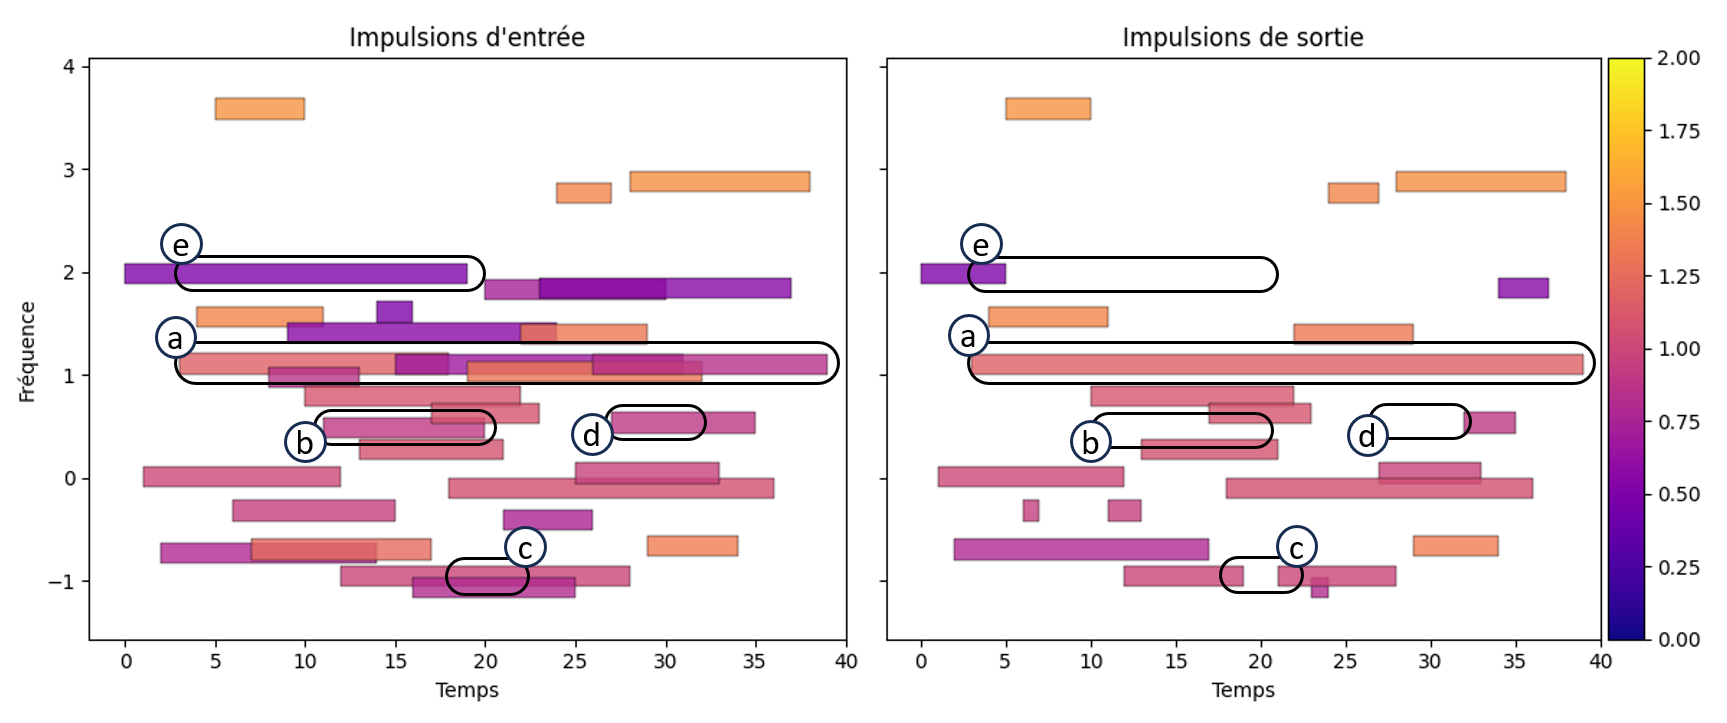
\includegraphics[scale=0.35]{IOsimpleexemple.png}
\end{center}
\caption{Représentation dans un plan temps-fréquence des PDW entrant dans le DCIS (à gauche) et sortant de ce module (à droite) simplifiant la modélisation du processus de DCI. La couleur de chaque rectangle encode l'amplitude du PDW. Les annotations identifient les dégradations structurelles induites par le traitement : (a) Fusion de signaux distincts, (b) Disparition d'impulsion (non-détection), (c) Scission artificielle d'une impulsion continue, (d) Troncature avant, (e) Troncature arrière, comme dans \ref{fig:IOex}}
\label{fig:IOsimple}
\end{figure}

Par conséquent, l'objectif d'optimisation de nos architectures d'apprentissage automatique reste inchangé. Nos modèles devront apprendre, à partir des seules données d'entrée/sortie, la transformation opérée par le DCIS, décrite dans ce chapitre, afin de prédire de manière causale la séquence des PDW interceptés. La fidélité des prédictions pourra être formellement évaluée non-seulement en calculant l'erreur quadratique entre PDW mais aussi en observant l'apparition des artéfacts aux endroits attendus.

\include{EUSIPCO}

\chapter*{L'approche séquence vers séquence}
\label{chap:seq2seq}
On introduit l'étude, on aborde les difficultés du problème de base et qu'on étudie ici un problème similaire simplifié.
\section*{Description du problème}
On introduit le problème simplifié, en insistant sur les modifications avec le problème de base et les apports de cette étude.
\subsection*{Encodage du temps}
\label{seq:timeencoding}
\begin{equation}
\label{eq:timeencodingin}
a = b + 1
\text{Ici on montre comment le temps est encodé dans les séquences}
\end{equation}

\begin{equation}
\label{eq:timeencodingout}
a = b + 1
\text{Ici on montre comment le temps est encodé dans les séquences}
\end{equation}
\section*{Architectures employées}
On introduit les architectures étudiées pour cette partie, il faut justifier ces choix. Il s'agit d'un transformer mais on pourra ajouter des résultats sur les RNNs permettant de les disqualifier. Les CNNs ne s'adapte pas au traitement seq2seq.
\section*{Suite : (ce n'est pas un titre de section}
Dans la suite on présentera comme dans la soumission à CAID.
\section*{Traitement de séquence entière}
\section*{Fenêtrage}
\section*{Discussion}
\label{seq:discseq2seq}


\chapter{L'approche séquence vers séquence}
Le chapitre présente la principale méthode de résolution de la problématique : une approche de transduction séquence ver séquence. Cette approche est la plus naturelle du point de vue de l'environnement virtuel puisque le module DCI génère toutes les impulsions avant que les modules suivantes ne traitent la séquence d'interceptions entière. Ce chapitre présente les travaux que constituent un article soumis à la conférence CAID. Il est articulé en trois sections. Nous commençons en exposant à nouveau les motivations de cette approches, en formulant nos attendes et nos réserves par rapport aux chances de succès. Ensuite nous présentons des travaux concernant le traitement des séquences entières, approches dont les limites sont liées aux tailles des séquences traitées. Finalement, nous présentons des travaux sur un mécanisme de fenêtrage, permettant de traiter les séquences longues en plusieurs fois, et son intégration dans un processus de prédiction de séquences.

\section{Motivations}
Les Transformers excellent 


\include{Stage}

\printbibliography

\end{document}
